% ============================================================================
% Fecha o Mês: um jogo sério de educação financeira com balanceamento por
% agentes automatizados
%
% Projeto para o Overleaf: suba a pasta inteira (main.tex, referencias.bib e
% figuras/). Compila com pdfLaTeX + BibTeX.
%
% Está em `article` para compilar em qualquer lugar. Para submeter na SBC
% (SBGames, SBIE, WEI), troque o preâmbulo pelo modelo oficial da SBC
% (sbc-template.sty) --- o corpo do texto já segue a estrutura deles.
%
% Marcadores [ASSIM] e % TODO são lugares para o time completar.
% Todos os números do texto saem do código e da rodada de robôs de
% 03/10/2026 (npm run bots -- --rooms 66 --seed 2026).
% ============================================================================
\documentclass[11pt,a4paper]{article}

\usepackage[T1]{fontenc}
\usepackage[utf8]{inputenc}
\usepackage[brazilian]{babel}
\usepackage{lmodern}
\usepackage[margin=2.5cm]{geometry}
\usepackage{graphicx}
\usepackage{booktabs}
\usepackage{tabularx}
\usepackage{array}
\usepackage{xcolor}
\usepackage{tikz}
\usetikzlibrary{arrows.meta,positioning,shapes.geometric,babel}
\usepackage{pgfplots}
\pgfplotsset{compat=1.18, /pgf/number format/use comma, /pgf/number format/1000 sep={.}}
\usepackage{caption}
\usepackage{subcaption}
\usepackage{enumitem}
\usepackage[numbers,sort&compress]{natbib}
\usepackage[hidelinks]{hyperref}

\definecolor{azul}{HTML}{2457C5}
\definecolor{rosa}{HTML}{D6337A}
\definecolor{verde}{HTML}{2B8C41}
\definecolor{ambar}{HTML}{B07A0C}
\definecolor{cinza}{HTML}{6B7A62}

\title{\textbf{Fecha o Mês}: um jogo sério de educação financeira\\com consequências encadeadas e balanceamento por agentes automatizados}
\author{[Autor 1]\thanks{[Instituição] --- [e-mail]} \and [Autor 2] \and [Autor 3] \and [Orientador(a)]}
\date{}

\begin{document}
\maketitle

\begin{abstract}
Decisões financeiras do dia a dia raramente têm efeito imediato: um empréstimo a um amigo, uma consulta adiada ou uma compra parcelada cobram seu preço meses depois. Apresentamos o \emph{Fecha o Mês}, um jogo sério multijogador para jovens adultos em que cada partida simula um ano de vida financeira de um recém-formado em uma cidade fictícia. A cada mês o jogador paga contas, escolhe um lazer, responde a um dilema e decide o que fazer com o dinheiro em produtos reais de renda fixa e variável; as escolhas geram consequências agendadas para meses futuros, reveladas apenas quando acontecem. Descrevemos o desenho do jogo, sua arquitetura e um método de balanceamento baseado em doze agentes com estratégias distintas, que jogam partidas completas pelas mesmas rotas do servidor usado por pessoas. Em 792 anos simulados, o método revelou dois defeitos que passavam por todos os testes automatizados, orientou o ajuste dos três caminhos de habilidade (de R\$~3.828 para R\$~82 de diferença no patrimônio anual) e mostrou que as decisões nos dilemas pesam cerca de três vezes mais no resultado do que a escolha de onde investir.

\medskip
\noindent\textbf{Palavras-chave:} jogos sérios; educação financeira; balanceamento de jogos; testes automatizados com agentes.
\end{abstract}

% ----------------------------------------------------------------------------
\section{Introdução}

A literacia financeira está associada a melhores decisões de poupança, endividamento e planejamento \cite{lusardi2014}, e uma meta-análise de 76 experimentos randomizados mostra que a educação financeira melhora tanto o conhecimento quanto o comportamento \cite{kaiser2022}. Ainda assim, no PISA 2022, 18\% dos estudantes dos países da OCDE ficaram abaixo do nível básico de letramento financeiro \cite{oecd2024}. No Brasil, a educação financeira aparece como tema transversal na Base Nacional Comum Curricular \cite{bncc2018} e é acompanhada pelo Banco Central \cite{bcb2021}; entre jovens de 18 a 25 anos, as negociações de dívida cresceram 49\% de janeiro a julho de 2025 \cite{serasa2025}.

Ensinar finanças por exposição tem um limite: as consequências de uma decisão financeira costumam aparecer muito depois dela, e é justamente essa distância entre escolha e efeito que favorece o adiamento \cite{odonoghue1999}. Jogos permitem viver essa distância em minutos, com a segurança de errar sem prejuízo real \cite{gee2003}.

Este trabalho nasceu como um projeto de iniciação científica para desenvolver um \emph{software de simulação do mercado financeiro}. Durante o projeto, o escopo foi redesenhado como um jogo: um simulador mostra produtos, mas um jogo consegue unir no mesmo ciclo orçamento, consumo, imprevistos, investimento, risco e consequências de longo prazo, e dar ao estudante um motivo para voltar a cada mês. O resultado é o \emph{Fecha o Mês}, um jogo para turmas em sala de aula, conduzido por um administrador (o professor), em que cada mês de jogo dura cerca de dez minutos. Nossas contribuições são:
\begin{enumerate}[leftmargin=*,itemsep=2pt]
  \item um ciclo mensal que combina obrigações (contas), escolhas de gosto (lazer), dilemas com \textbf{consequências agendadas} e investimentos com regras de produtos reais, fundamentado em teorias de motivação e aprendizagem;
  \item uma arquitetura em que toda a matemática financeira vive em funções puras, testadas isoladamente;
  \item um método de \textbf{balanceamento por agentes} que jogam pelo servidor real, com um agente de controle para medir o efeito de cada decisão isoladamente.
\end{enumerate}

% ----------------------------------------------------------------------------
\section{Referencial teórico}

\subsection{Jogos sérios e gamificação}

\citet{abt1970} cunhou o termo \emph{jogo sério} para jogos com propósito educacional explícito que não deixam de ser divertidos; \citet{michael2006} o ampliam para jogos que educam, treinam e informam. A \emph{gamificação}, por sua vez, é o uso de elementos de design de jogos em contextos que não são jogos \cite{deterding2011}: pontos, emblemas, rankings e níveis aplicados a uma atividade existente \cite{werbach2012}, com uso crescente na educação \cite{kapp2012}. A distinção importa para este trabalho. O \emph{Fecha o Mês} não acrescenta pontos a uma aula de finanças: é um jogo completo, com regras, objetivo e consequências, que \emph{também} usa elementos de gamificação (árvore de habilidades, conquistas, ranking).

A evidência empírica é favorável, com ressalvas. Em revisão de estudos empíricos, \citet{hamari2014} encontram efeitos em geral positivos da gamificação, mas dependentes do contexto e de quem usa. A revisão sistemática de \citet{connolly2012}, com 129 estudos, associa jogos sérios à aquisição de conhecimento e a efeitos motivacionais em pessoas a partir de 14 anos.

\subsection{Motivação e aprendizagem}

A Teoria da Autodeterminação \cite{ryan2000} explica a motivação intrínseca pela satisfação de três necessidades: autonomia, competência e pertencimento. \citet{sailer2017} mostram experimentalmente que elementos específicos atendem a necessidades específicas: emblemas e rankings à competência; história e colegas de equipe ao pertencimento. O estado de \emph{fluxo} \cite{csikszentmihalyi1990}, em que desafio e habilidade se equilibram, justifica a preocupação com o balanceamento. O ciclo da aprendizagem experiencial \cite{kolb1984} --- experiência, reflexão, conceituação e nova experimentação --- descreve bem um jogo em turnos, e a aprendizagem baseada em jogos digitais \cite{prensky2001,gee2003} aponta princípios como identidade, risco seguro e retorno imediato. Para descrever o jogo, usamos o modelo MDA \cite{hunicke2004}: as \emph{mecânicas} (contas, produtos, dilemas) geram \emph{dinâmicas} (endividamento, poupança, efeito diferido) que produzem \emph{estéticas} (desafio, descoberta, fantasia de vida adulta). A Tabela~\ref{tab:teoria} liga cada referência a uma mecânica do jogo.

\begin{table}[ht]
  \centering\small
  \caption{Fundamentos teóricos e onde aparecem no jogo.}
  \label{tab:teoria}
  \begin{tabularx}{\linewidth}{@{}l X@{}}
    \toprule
    Fundamento & Mecânica no Fecha o Mês \\
    \midrule
    Autonomia \cite{ryan2000} & escolher o lazer, o dom, o caminho de habilidades e onde investir \\
    Competência \cite{ryan2000,sailer2017} & patrimônio mês a mês, conquistas e ranking da sala \\
    Pertencimento \cite{ryan2000,sailer2017} & partida em turma, com o mesmo calendário para todos \\
    Fluxo \cite{csikszentmihalyi1990} & balanceamento por agentes; nenhum caminho dominante \\
    Ciclo experiencial \cite{kolb1984} & decidir (dilema), viver a consequência (virada), refletir (linha do tempo), decidir de novo \\
    Risco seguro \cite{gee2003} & dívida, demissão e calote sem prejuízo real \\
    MDA \cite{hunicke2004} & produtos reais (mecânica) $\rightarrow$ juros compostos (dinâmica) $\rightarrow$ descoberta (estética) \\
    \bottomrule
  \end{tabularx}
\end{table}

\subsection{Jogos de educação financeira}

No Brasil, o mapeamento sistemático de \citet{torrens2021} sobre jogos sérios de educação financeira aponta o modo multijogador e o uso de técnicas de inteligência artificial como lacunas da área. Um exemplo recente é o \emph{Grana} \cite{cavalcante2021}, jogo para dispositivos móveis voltado a crianças de escolas rurais. A revisão de \citet{andrade2025} conclui que jogos são eficazes em educação financeira, mas que medir o impacto no comportamento ainda é difícil. Em âmbito internacional, \citet{kalmi2021} discutem o potencial e os limites de jogos digitais, de tabuleiro e de interpretação de papéis na educação financeira. Fora da academia, o \emph{Cashflow 101} \cite{cashflow1996} popularizou o tema em tabuleiro, com foco em investimentos e fluxo de caixa, e o \emph{Spent} \cite{spent2011} simula sobreviver um mês com orçamento apertado, escolhendo entre contas. % TODO: incluir a referência do mural quando houver autores e ano.

O \emph{Fecha o Mês} se posiciona em três pontos dessa paisagem: é multijogador e conduzido em sala, respondendo à primeira lacuna de \citet{torrens2021}; trata as consequências diferidas como mecânica central, em vez de feedback imediato; e usa agentes automatizados no próprio processo de design, o que toca a segunda lacuna.

\subsection{Teste automatizado e balanceamento}

A indústria de jogos ainda depende quase só de testes manuais \cite{politowski2021}. Agentes que jogam com estilos diferentes já foram usados para testar fases e ajustar parâmetros: \citet{holmgard2019} propõem \emph{personas procedurais} que representam estilos de decisão, e \citet{zook2014} usam testes automáticos para ajustar parâmetros de jogo. Nossa abordagem é mais simples (agentes por regras, não aprendidos), mas joga pelo servidor de produção e adiciona um agente de controle para isolar o efeito de cada decisão.

% ----------------------------------------------------------------------------
\section{O jogo}

O jogador é um engenheiro recém-formado que se muda para Santa Rita, uma cidade fictícia. Ele recebe R\$~7.000 de salário por mês e começa com o salário de janeiro mais um presente de R\$~500 da família. A partida dura de janeiro a dezembro; vence quem termina com o maior \textbf{patrimônio líquido} --- saldo, aplicações e ações, menos cheque especial e parcelas a vencer. A cidade é o próprio menu (Figura~\ref{fig:mapa}): cada prédio é uma empresa com nome e história, e o mapa muda com as estações e o clima de cada mês.

\begin{figure}[ht]
  \centering
  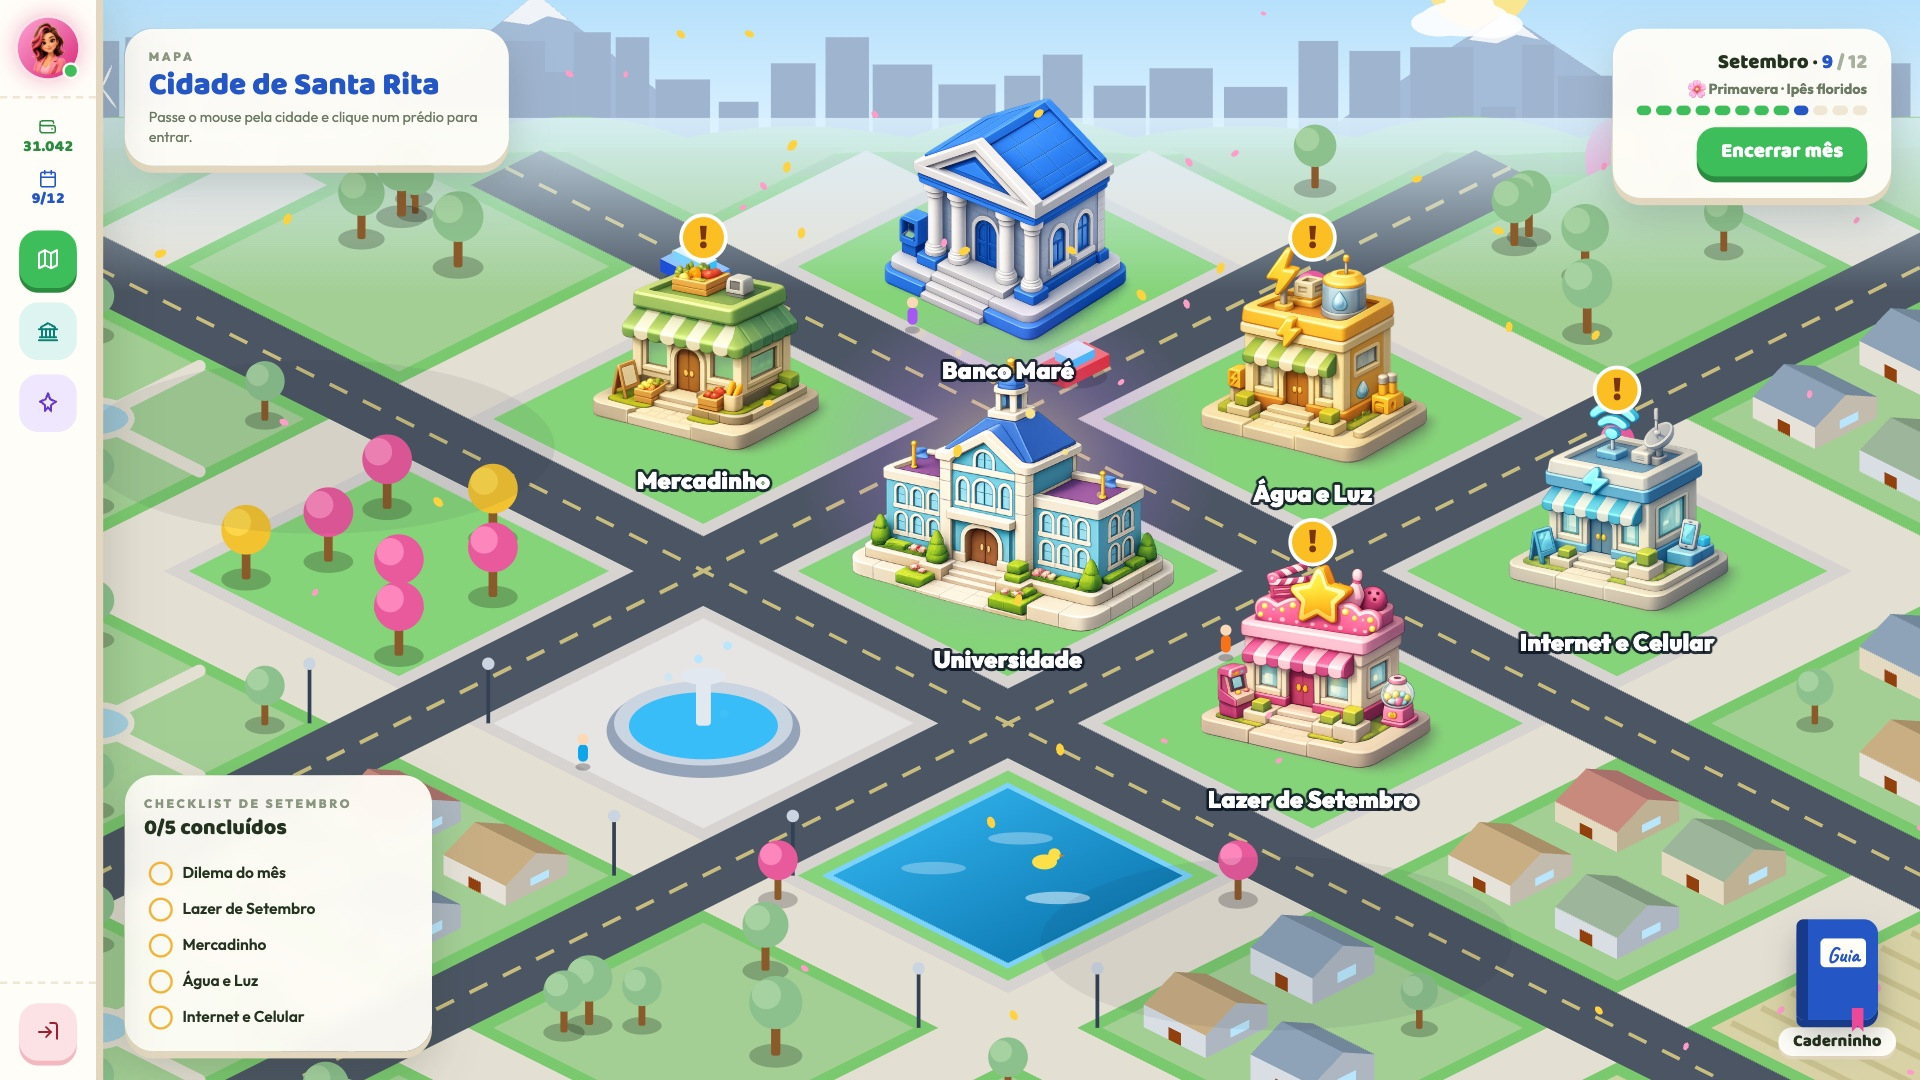
\includegraphics[width=\linewidth]{figuras/mapa.jpg}
  \caption{O mapa em setembro. Os prédios levam ao banco, às contas, ao lazer e à Universidade; à esquerda, a lista do que falta no mês; no canto, o caderninho.}
  \label{fig:mapa}
\end{figure}

\subsection{O ciclo mensal}

Cada mês segue o mesmo ciclo (Figura~\ref{fig:ciclo}). Na \textbf{virada}, o servidor cobra os juros do cheque especial sobre o saldo negativo, paga o salário, aplica as consequências marcadas para aquele mês, cobra o aluguel e sorteia o evento do mês. O jogador vê tudo isso em um cartão de resumo (Figura~\ref{fig:telas}a) e então responde ao dilema, escolhe o lazer, paga as três contas e decide o que fazer com o dinheiro no banco. O administrador fecha o mês quando a turma termina.

\begin{figure}[ht]
  \centering
  \begin{tikzpicture}[
    node distance=6mm and 4mm,
    passo/.style={draw=azul, rounded corners=4pt, fill=azul!8, minimum width=21mm, minimum height=10mm, align=center, font=\small},
    seta/.style={-{Stealth[length=2.5mm]}, thick, azul}
  ]
    \node[passo, fill=azul!25] (v) {Virada};
    \node[passo, right=of v] (d) {Dilema};
    \node[passo, right=of d] (l) {Lazer};
    \node[passo, right=of l] (c) {Contas};
    \node[passo, right=of c] (b) {Banco};
    \node[passo, right=of b] (e) {Encerrar};
    \draw[seta] (v) -- (d); \draw[seta] (d) -- (l); \draw[seta] (l) -- (c); \draw[seta] (c) -- (b); \draw[seta] (b) -- (e);
    \draw[seta] (e.south) -- ++(0,-7mm) -| node[pos=0.25, below, font=\footnotesize, text=cinza] {o administrador fecha o mês; o que ficou em aberto é cobrado} (v.south);
  \end{tikzpicture}
  \caption{O ciclo de um mês.}
  \label{fig:ciclo}
\end{figure}

\paragraph{Nada fica de graça.} Se o mês fecha com algo pendente, a virada cobra: conta não paga vira \emph{conta atrasada}, com 2\% de multa e 1\% de juros; o lazer não escolhido é cobrado; e o dilema sem resposta é decidido pela \emph{inércia}, a opção de quem não fez nada. Essa regra nasceu do balanceamento (Seção~\ref{sec:resultados}).

\subsection{Dilemas e consequências encadeadas}

Há onze dilemas, de janeiro a novembro, cada um com duas opções. O jogador vê o custo imediato de cada opção, quanto sobraria na conta e o total guardado nas aplicações, mas nunca a consequência (Figura~\ref{fig:telas}b): ela é agendada no servidor e revelada na virada do mês em que acontece. A resposta pode ser adiada dentro do mês, para que o jogador consulte o banco e as contas antes de decidir --- planejar é parte do que o jogo ensina. A Tabela~\ref{tab:consequencias} mostra algumas cadeias. Algumas consequências dependem de mais de uma escolha: quem vai a pé para o trabalho em agosto e falta ao programa de TV em setembro é demitido em novembro e fica sem o salário de dezembro.

\begin{table}[ht]
  \centering\small
  \caption{Exemplos de consequências agendadas.}
  \label{tab:consequencias}
  \begin{tabularx}{\linewidth}{@{}l X X r@{}}
    \toprule
    Mês & Escolha & Consequência & Valor \\
    \midrule
    Fev & Emprestar R\$~500 a um amigo & devolvidos em maio, com agradecimento & $+$537 \\
    Mar & Adiar o dentista & tratamento de canal em junho & $-$500 \\
    Abr & Parcelar a máquina em 12$\times$ & parcelas até dezembro; 3 restam como dívida & $-$4.022 \\
    Jun & Seguir trabalhando exausto & crise de coluna em agosto & $-$2.000 \\
    Ago e Set & Ir a pé e faltar à TV & demissão; dezembro sem salário & $-$7.000 \\
    Set & Ir ao programa de TV & promoção de outubro a dezembro & $+$2.100 \\
    Nov & Processar a loja & ganha a causa em dezembro & $+$5.000 \\
    \bottomrule
  \end{tabularx}
\end{table}

Parcelas que passam do fim do ano entram como dívida no patrimônio. Sem essa regra, parcelar a máquina sairia mais barato que pagar à vista (R\$~3.016,80 pagos no ano contra R\$~3.620), e o jogo ensinaria o contrário do pretendido.

\subsection{Eventos, lazer e dinheiro}

\paragraph{Eventos.} Cada mês tem um calendário próprio de imprevistos sem escolha (casamento de um amigo, restituição do IR, celular quebrado, participação nos resultados, décimo terceiro). Em cada virada sorteia-se um da lista do mês, ou nenhum com 20\% de chance.

\paragraph{Lazer.} Duas opções com o mesmo preço por mês (por exemplo, kart ou boliche). A escolha é de gosto, não de dinheiro, mas o lazer é obrigatório e soma R\$~4.850 no ano.

\paragraph{Banco.} O banco oferece poupança, CDB, Tesouro Selic, Tesouro Prefixado, LCI, LCA, uma debênture e quatro ações, com rentabilidade, liquidez, prazo e imposto de renda segundo uma tabela de referência do projeto (Selic simulada de 10,5\% e CDI de 10,4\% ao ano). Saldo negativo é cheque especial a 8\% ao mês.

\subsection{Personagem, habilidades e descoberta}

Na criação, o jogador escolhe um de três \emph{dons} (custos fixos 10\% menores; um freela mensal e eventos positivos maiores; ou mais pontos de habilidade). Cada dilema respondido dá um ponto para a Universidade, uma constelação de doze habilidades em três caminhos --- Técnico (renda), Comunicação (descontos) e Gestão (bônus sobre o que se guarda). Três cupons escondidos no mapa, um por fase do ano, premiam quem explora. Um \emph{caderninho} sempre disponível explica como jogar e traz um glossário de 21 termos (Figura~\ref{fig:telas}c); a tela final mostra o pódio, as conquistas e a linha do tempo das escolhas e de suas consequências (Figura~\ref{fig:telas}d).

\begin{figure}[ht]
  \centering
  \begin{subfigure}{0.49\linewidth}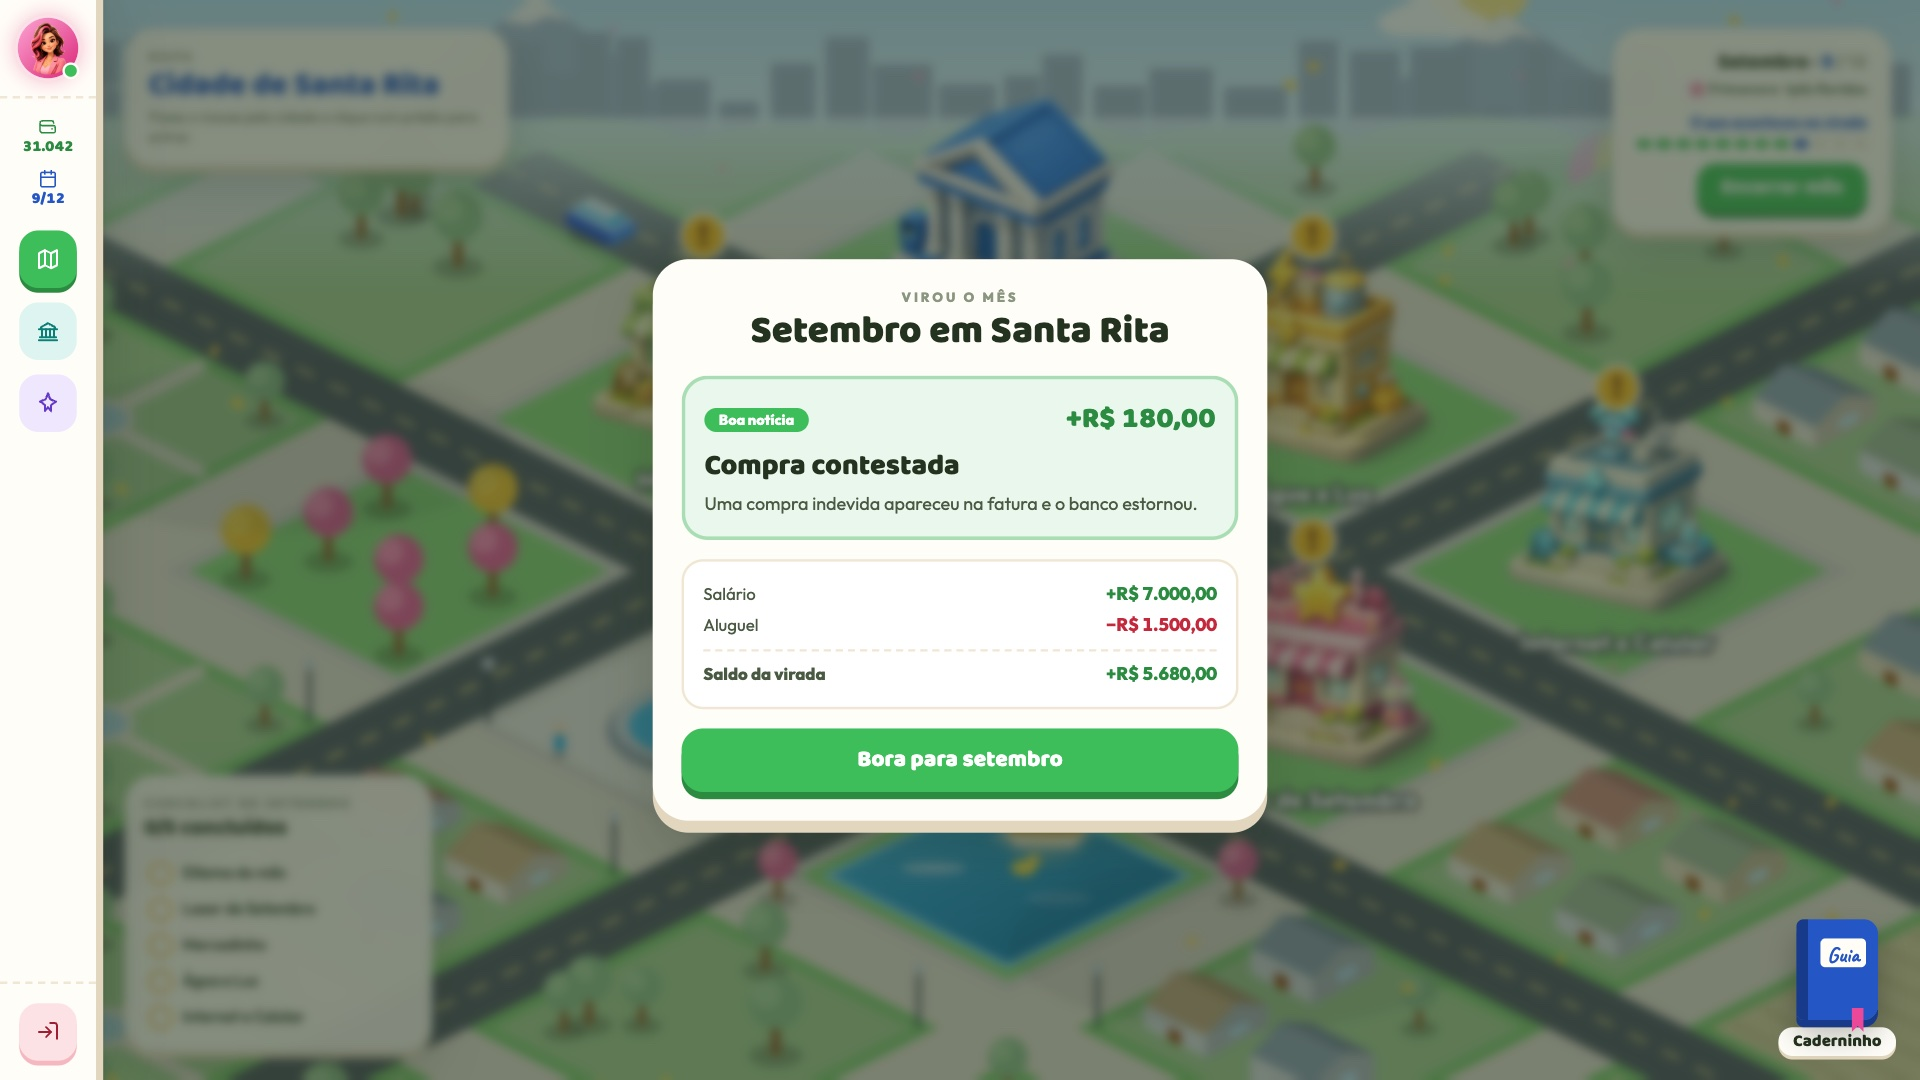
\includegraphics[width=\linewidth]{figuras/virada.jpg}\caption{Resumo da virada}\end{subfigure}\hfill
  \begin{subfigure}{0.49\linewidth}
\includegraphics[width=\linewidth]{figuras/dilema.jpg}\caption{Dilema de setembro}\end{subfigure}\\[2mm]
  \begin{subfigure}{0.49\linewidth}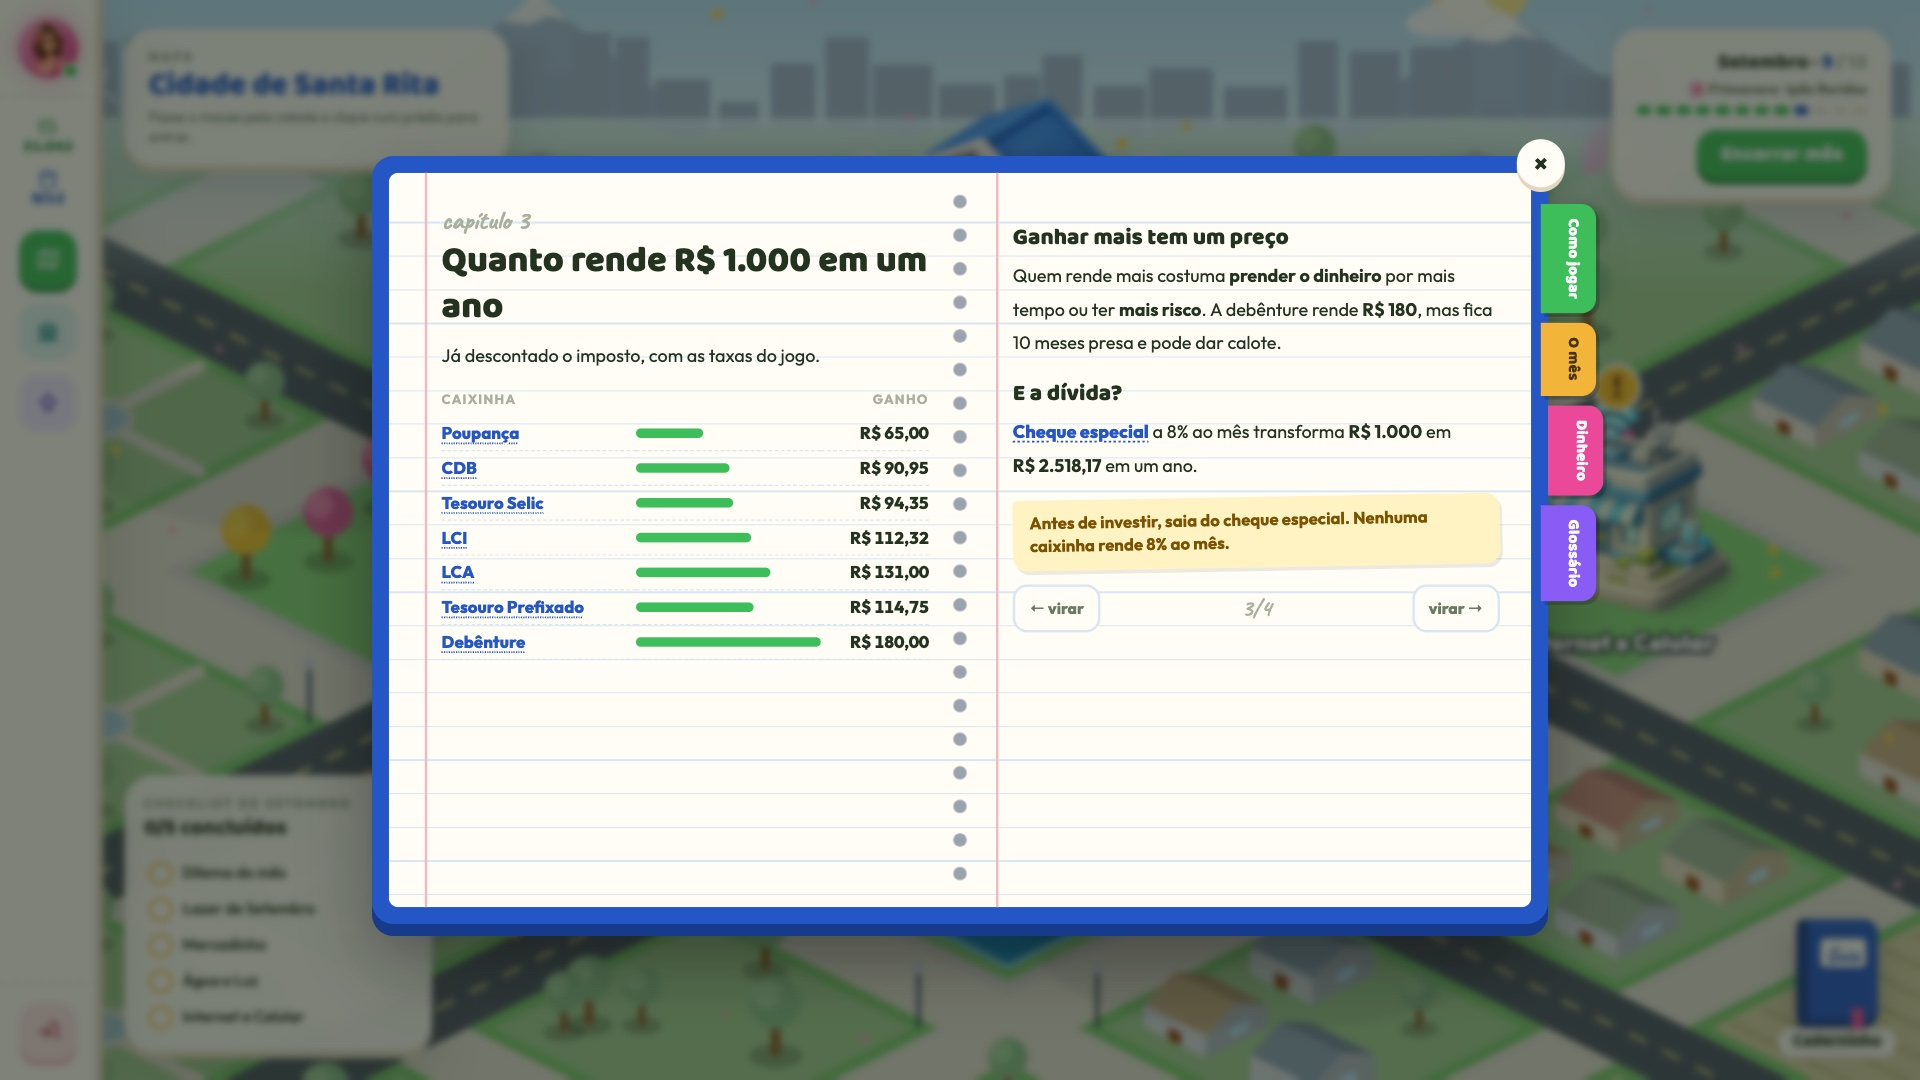
\includegraphics[width=\linewidth]{figuras/caderninho.jpg}\caption{Caderninho}\end{subfigure}\hfill
  \begin{subfigure}{0.49\linewidth}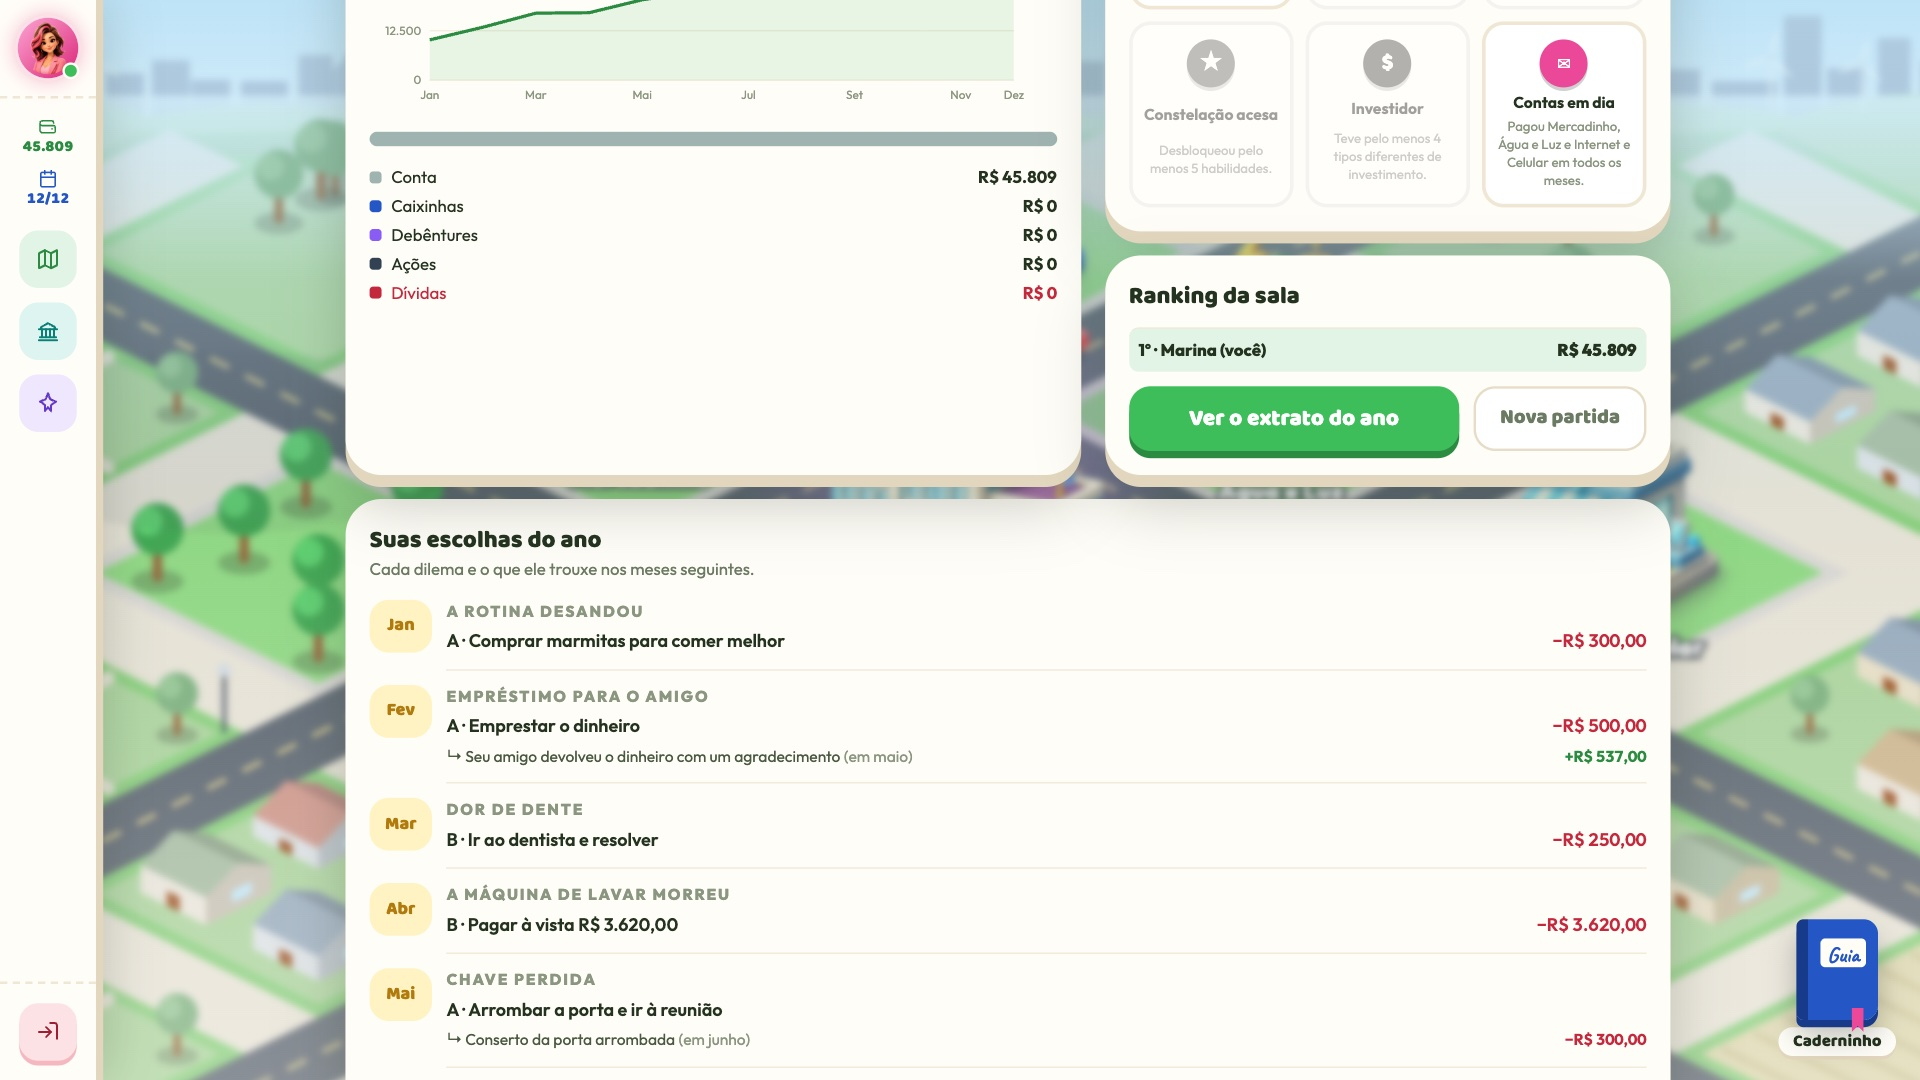
\includegraphics[width=\linewidth]{figuras/linha-do-tempo.jpg}\caption{Linha do tempo no fim do ano}\end{subfigure}
  \caption{Telas do jogo.}
  \label{fig:telas}
\end{figure}

\subsection{O papel do professor}

O administrador cria uma sala por turma, distribui o código e acompanha, em tempo real, o que falta para cada jogador no mês (Figura~\ref{fig:admin}). Fechar o mês com alunos pendentes pede confirmação. O cadastro de administrador exige um código de convite.

\begin{figure}[ht]
  \centering
  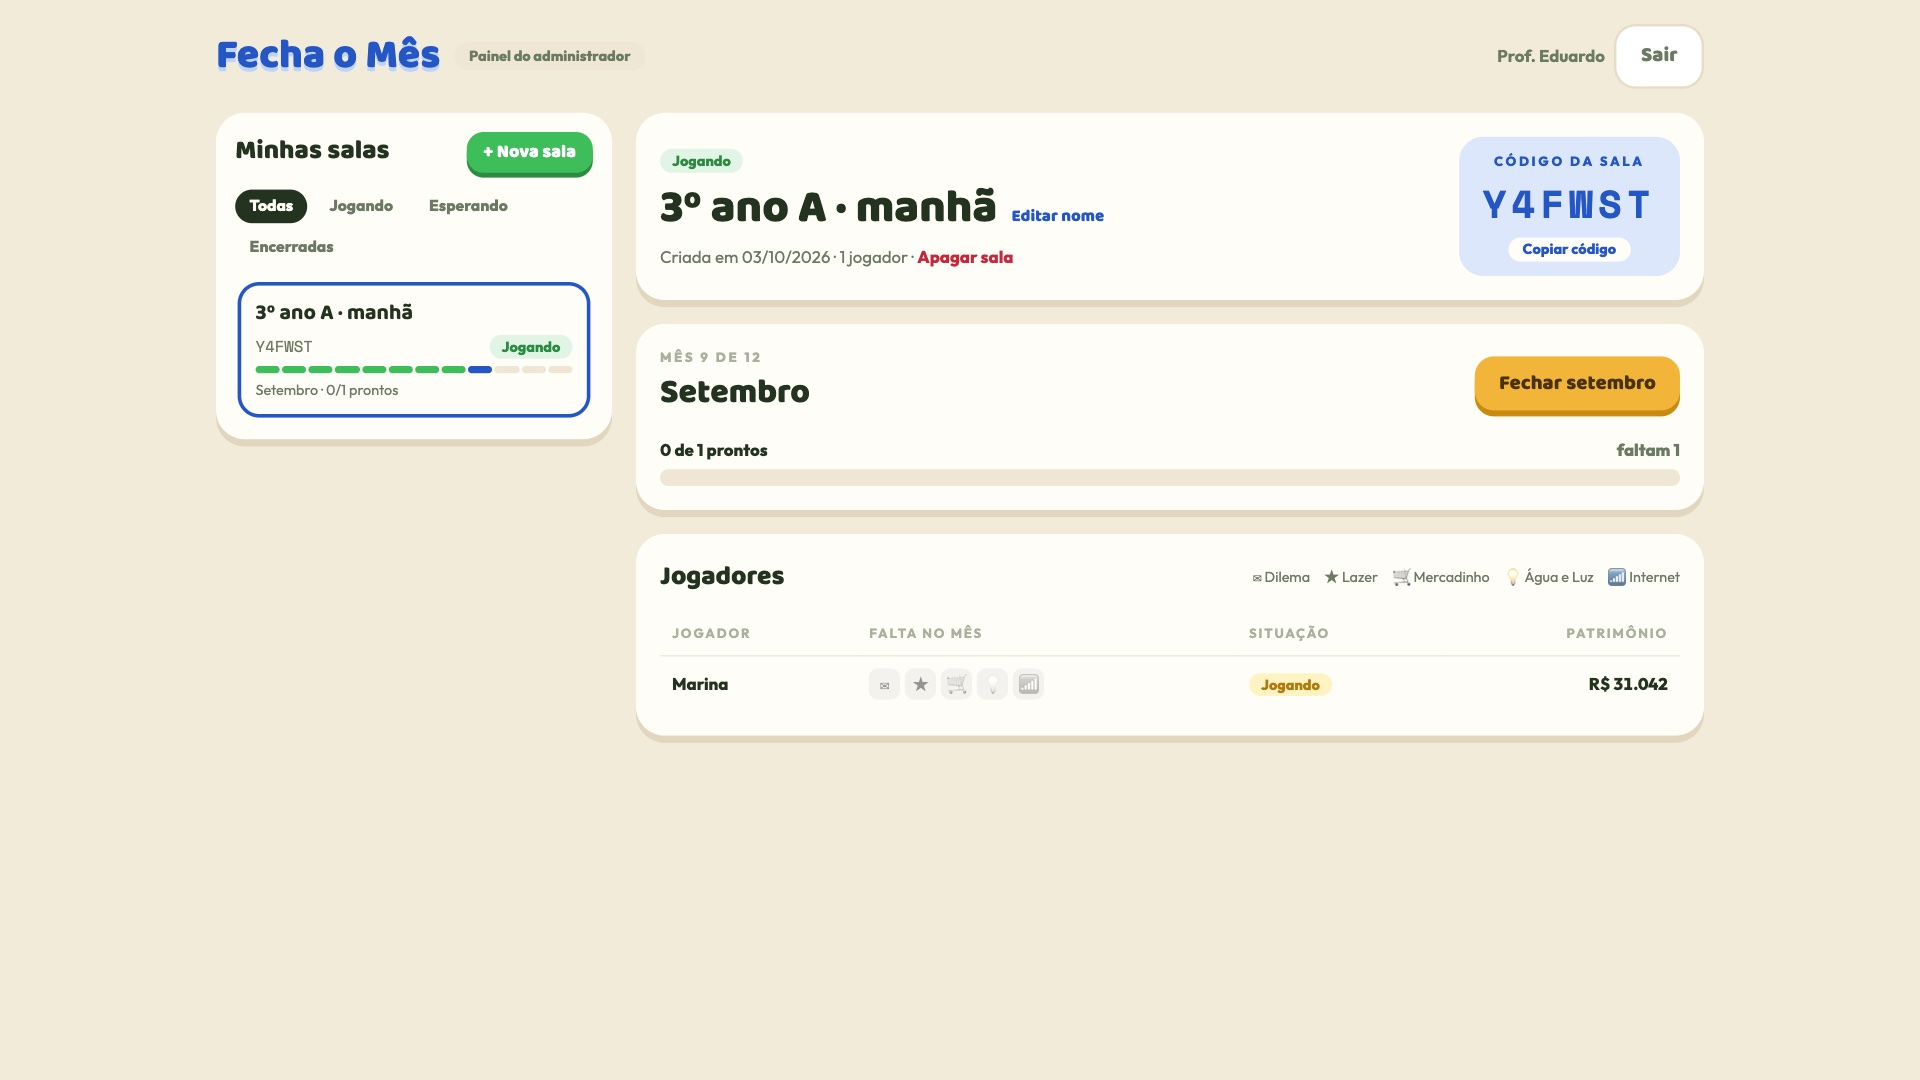
\includegraphics[width=0.85\linewidth]{figuras/painel-admin.jpg}
  \caption{Painel do administrador: salas da turma e progresso de cada jogador no mês.}
  \label{fig:admin}
\end{figure}

% ----------------------------------------------------------------------------
\section{Arquitetura e implementação}

O cliente é uma aplicação React~19 com Vite, Tailwind CSS e Framer Motion; o estado global usa Zustand. O servidor é Node.js com Express~5, Prisma~5 sobre SQLite (Turso em produção) e Socket.IO para avisar a turma quando o mês vira.

\paragraph{Matemática em funções puras.} Toda regra de dinheiro --- juros, cheque especial, imposto de renda, rendimento das aplicações, dilemas, consequências, eventos e cobrança do que ficou em aberto --- está em módulos sem acesso a banco de dados. O motor de turnos apenas lê o estado, chama essas funções e grava o resultado. Isso permite testar cada regra isoladamente e reutilizá-la no cliente.

\paragraph{Consequências agendadas.} Ao responder um dilema, o servidor grava a escolha e as consequências futuras numa tabela de efeitos (mês de aplicação, tipo, valor e rótulo). Na virada, o motor aplica os efeitos daquele mês e os marca como aplicados; efeitos depois de dezembro permanecem como dívida. Tipos de efeito cobrem dinheiro, parcelas, aumento de salário, mês sem salário, aluguel já pago e avisos.

\paragraph{Testes.} O projeto tem 1.077 testes automatizados no servidor e 113 no cliente, cobrindo as regras financeiras, as rotas e as permissões. % TODO: cobertura de código, se o time quiser relatar.

% ----------------------------------------------------------------------------
\section{Balanceamento com agentes}
\label{sec:metodo}

Testes unitários verificam cada regra isoladamente, mas não respondem se o jogo como um todo recompensa as decisões certas. Para isso, criamos doze agentes por regras (Tabela~\ref{tab:agentes}) que jogam partidas completas.

\begin{table}[ht]
  \centering\small
  \caption{Os agentes. ``Prudente'' e ``descuidado'' são roteiros fixos de respostas aos dilemas; ``esperto'' é o roteiro de maior retorno em dinheiro.}
  \label{tab:agentes}
  \begin{tabularx}{\linewidth}{@{}l l X@{}}
    \toprule
    Agente & Dilemas & Dinheiro \\
    \midrule
    Zé Gastão & mais barato agora & não investe \\
    Dona Formiga & prudente & poupança \\
    Tia Planilha & esperto & diversifica (LCA, Tesouro, CDB, debênture, ações) \\
    Lobinho da Bolsa & aleatório & 80\% em ações \\
    Seu Parcelinha & descuidado & não investe \\
    Prudêncio & prudente & reserva de 3 meses; resto em LCA \\
    Sorte Grande & aleatório & poupança \\
    Cuponete & esperto & CDB; procura os cupons \\
    Dr.\ Juros & esperto & só isentos de IR (LCA e LCI) \\
    Debi Debênture & prudente & 60\% em debênture \\
    Seu Cofrinho & prudente & \textbf{controle}: não investe \\
    Dorminhoco & não responde & não faz nada \\
    \bottomrule
  \end{tabularx}
\end{table}

\paragraph{Execução.} Os agentes usam as mesmas rotas HTTP do jogo, contra uma cópia do banco de dados sem partidas, com um administrador também automatizado que abre salas e fecha os meses. O gerador pseudoaleatório do servidor recebe uma semente fixa, o que torna qualquer rodada reprodutível. Em cada sala, os doze agentes jogam juntos; o dom e o caminho de habilidade de cada agente giram entre as salas, de modo que todos passam por todas as combinações.

\paragraph{Comparações controladas.} Como cada agente combina uma política de dilemas com uma de investimento, comparar agentes quaisquer mistura efeitos. Medimos cada decisão comparando agentes que diferem só nela: dilemas, pelo Seu Cofrinho contra o Seu Parcelinha (nenhum investe); investir, pelo melhor investidor prudente contra o Seu Cofrinho (mesmos dilemas); ações sem informação, pelo Lobinho contra o Sorte Grande (ambos decidem ao acaso). Dons e caminhos são comparados apenas entre agentes que investem.

% ----------------------------------------------------------------------------
\section{Resultados}
\label{sec:resultados}

A rodada final teve 66 salas, ou 792 anos jogados, em 441 segundos, sem nenhum erro do servidor. A Figura~\ref{fig:ranking} mostra o patrimônio final médio por agente.

\begin{figure}[ht]
  \centering
  \begin{tikzpicture}
    \begin{axis}[
      xbar, width=0.82\linewidth, height=8.2cm, bar width=7pt,
      xmin=0, xmax=72, xlabel={Patrimônio médio em dezembro (R\$ mil)},
      ytick={1,...,12},
      yticklabels={Dorminhoco, Zé Gastão, Seu Parcelinha, Lobinho da Bolsa, Sorte Grande, Seu Cofrinho, Debi Debênture, Tia Planilha, Prudêncio, Dona Formiga, Dr.\ Juros, Cuponete},
      y tick label style={font=\small}, x tick label style={font=\small},
      nodes near coords, nodes near coords style={font=\scriptsize, /pgf/number format/fixed, /pgf/number format/precision=1},
      axis x line*=bottom, axis y line*=left, enlarge y limits=0.06
    ]
      \addplot[fill=azul!70, draw=none] coordinates {
        (32.5,1) (41.1,2) (41.2,3) (50.2,4) (55.8,5) (57.8,6) (61.8,7) (62.0,8) (62.2,9) (62.7,10) (64.0,11) (64.7,12)
      };
    \end{axis}
  \end{tikzpicture}
  \caption{Patrimônio final médio de cada agente em 66 salas (semente 2026).}
  \label{fig:ranking}
\end{figure}

\paragraph{O que decide o resultado.} As comparações controladas (Figura~\ref{fig:peso}) mostram que decidir com cuidado nos dilemas vale R\$~16.639 a mais no ano, cerca de três vezes o ganho de investir em vez de deixar o dinheiro parado (R\$~4.923). Comprar ações todo mês sem informação custou R\$~5.536 em relação à poupança, em grande parte por um evento de mercado agendado (queda de 35\% de uma das ações em outubro). Dons e caminhos de habilidade, depois do ajuste, pesam menos de 1\%.

\begin{figure}[ht]
  \centering
  \begin{tikzpicture}
    \begin{axis}[
      xbar, width=0.7\linewidth, height=5.2cm, bar width=9pt,
      xmin=0, xmax=19500, xlabel={Diferença no patrimônio anual (R\$)},
      ytick={1,...,5},
      yticklabels={Caminho da Universidade, Dom, Investir ou deixar na conta, Ações às cegas ou poupança, Dilemas: cuidado ou descuido},
      y tick label style={font=\small}, x tick label style={font=\small},
      scaled x ticks=false, xtick={0,4000,8000,12000,16000},
      nodes near coords, nodes near coords style={font=\scriptsize},
      axis x line*=bottom, axis y line*=left, enlarge y limits=0.12
    ]
      \addplot[fill=rosa!75, draw=none] coordinates {
        (82,1) (371,2) (4923,3) (5536,4) (16639,5)
      };
    \end{axis}
  \end{tikzpicture}
  \caption{Peso de cada decisão, medido entre agentes que diferem apenas nela.}
  \label{fig:peso}
\end{figure}

\paragraph{Ajuste dos caminhos de habilidade.} Na primeira medição, entre agentes que investem, o caminho de Comunicação terminava R\$~3.828 à frente do de Gestão, cujo bônus depende do saldo aplicado. Testamos em paralelo multiplicadores de 1, 1,5, 2 e 2,5 sobre o bônus da Gestão; o efeito foi aproximadamente linear (cerca de R\$~3.200 a cada 0,5). O ajuste final combinou Gestão $\times$1,4 com pequenas mudanças nos outros dois caminhos, e a diferença caiu para R\$~82 (Tabela~\ref{tab:caminhos}). Os três dons ficaram a R\$~371 um do outro.

\begin{table}[ht]
  \centering\small
  \caption{Patrimônio médio por caminho, entre agentes que investem. Antes: 27 salas (semente 77). Depois: 66 salas (semente 2026).}
  \label{tab:caminhos}
  \begin{tabular}{@{}lrr@{}}
    \toprule
    Caminho & Antes (R\$) & Depois (R\$) \\
    \midrule
    Técnico & 58.480 & 60.457 \\
    Comunicação & 61.110 & 60.461 \\
    Gestão & 57.282 & 60.379 \\
    \midrule
    Maior diferença & 3.828 & 82 \\
    \bottomrule
  \end{tabular}
\end{table}

\paragraph{Defeitos encontrados.} Os agentes revelaram dois defeitos que passavam por todos os testes. (i) O agente que não fazia nada terminava em primeiro lugar, porque contas não pagas nunca eram cobradas; a correção (cobrança na virada com multa e juros, lazer e inércia) o levou ao último lugar. (ii) O patrimônio registrado a cada mês, usado no ranking final, ignorava as ações, prejudicando quem investia em bolsa. Também ficou visível que os eventos só apareciam no extrato do banco, o que motivou o cartão de resumo da virada.

% ----------------------------------------------------------------------------
\section{Discussão e limitações}

Os resultados indicam que o jogo recompensa decisão, não sorte de largada: escolher bem nos dilemas pesa muito mais que o dom ou o caminho de habilidade. Ao mesmo tempo, nenhum agente entrou no cheque especial em nenhum mês: o salário sobra entre R\$~3 e 4 mil depois das contas, o que sugere que o orçamento está folgado demais para ensinar sobre dívida. % TODO: decisão do time sobre apertar o orçamento.

Há limitações importantes. Os agentes seguem regras fixas e não aprendem, então medem o espaço de estratégias que escolhemos, não o de pessoas reais. A inflação não é modelada: os preços ficam constantes no ano. E, principalmente, este trabalho ainda não avalia o aprendizado com estudantes.

% ----------------------------------------------------------------------------
\section{Conclusão e trabalhos futuros}

Apresentamos o Fecha o Mês, um jogo sério de educação financeira com consequências encadeadas, e um método de balanceamento por agentes que jogam pelo servidor real. O método encontrou defeitos invisíveis aos testes unitários, guiou o ajuste fino das habilidades e quantificou o peso de cada decisão. Como próximos passos, planejamos: [um estudo com turmas, com pré e pós-teste de literacia financeira baseado em instrumento validado]; ajustar o orçamento para que a dívida apareça no jogo; e agentes que aprendam estratégias, para buscar desequilíbrios que não imaginamos. % TODO: desenho do estudo com estudantes.

\bibliographystyle{plainnat}
\bibliography{referencias}

\end{document}
